\documentclass[aps,twocolumn,nobalancelastpage,amsmath,amssymb,
nofootinbib,superscriptaddress, ]{revtex4}
%secnumarabic


% nofootinbib is another document class option that allows you to put poop
% footnotes on the page where they occur rather than at the end of the
% paper.  This makes for easier reading!

% secnumarabic is a particularly nice way of identifying sections by
% number to aid electronic review and commentary.

% amsmath and amssymb are necessary for the subequations environment
% among others

\usepackage{graphics}      % standard graphics specifications
\usepackage{graphicx}      % alternative graphics specifications
\usepackage{longtable}     % helps with long table options
\usepackage{url}           % for on-line citations
\usepackage{bm}            % special 'bold-math' package
\usepackage{courier}
%\usepackage{verbatim}   % useful for program listings
%\usepackage{color}      % use if color is used in text
%\usepackage{subfigure}  % use for side-by-side figures
%\usepackage{hyperref}   % use for hypertext links, including those to external documents and URLs
%\raggedbottom           % don't add extra vertical space
\DeclareGraphicsExtensions{.pdf}


\begin{document}
\title{Statistical risk analysis and the development of robust distributed applications for NASA's Deep Space Network}
\author         {Ian W. \surname{Bornhoeft}}
\email          {bornhi@rpi.edu}
\homepage       {http://www.jpl.nasa.gov}
\affiliation{Jet Propulsion Laboratory, California Institute of Technology, 4800 Oak Grove Dr, Pasadena, CA 91109}
\affiliation{Department of Physics, Applied Physics, and Astronomy, Rensselaer Polytechnic Institute, 110 8th St, Troy, NY 12180}
\author         {Silvino C. \surname{Zendejas}}
\email          {silvino.c.zendejas@jpl.nasa.gov}
\homepage       {http://www.jpl.nasa.gov}
\affiliation{Jet Propulsion Laboratory, California Institute of Technology, 4800 Oak Grove Dr, Pasadena, CA 91109}
\author         {Paul A. \surname{Wolgast}}
\email          {paul.a.wolgast@jpl.nasa.gov}
\homepage       {http://www.jpl.nasa.gov}
\affiliation{Jet Propulsion Laboratory, California Institute of Technology, 4800 Oak Grove Dr, Pasadena, CA 91109}
\date{August 19, 2013} %\today}

\begin{abstract}
Deep Space Network (DSN) equipment failures can cripple NASA’s telecommunication service capabilities and result in irreversible data losses during mission nominal and critical events. The continuous effort to make the DSN more operationally efficient and less costly to operate, introduces challenges in the ground data system software architecture and the ability to manage risk effectively. The concepts behind relational databases and the tools provided by the Structured Query Language (SQL) in Oracle, provide a means for quantifying the risk of data loss under various conditions involving different levels of automation. The concepts behind the development of the Erlang programming language, designed to address the needs of robust, reliable, and efficient telecommunication software solutions, can be applied to specific functional areas of the DSN Service Management System (DSMS). Using a combination of predictive methods based on analyses of historical DSN error data and more robust distributed software architectures developed with Erlang, it is possible to make the DSN more reliable and operationally efficient.
\end{abstract}

\maketitle


%%%%%%%%%%%%%%%%%%%%%%%%%%%%%%%%%%%%%%%%%%%%%%%%%%%%%%%%%%%%%%%%%%%%%%%%%%%%%%
\section{Introduction}

The Deep Space Network (DSN) has been in operation since 1959, and most of its antennas were built in the 1960s and 1970s. Although five new antennas were added in the 1990s and one in 2003, the DSN is aging and, combined with the fact that the DSN is supporting more missions at further distances from the Earth than it was originally designed to handle, equipment failures, while still remaining relatively infrequent, have become more incessant and detrimental in recent years. \cite{bagri2007} \cite{wackley2011} It is therefore more necessary than ever for methodologies to be in place which can handle such failures when they occur.

In this investigation, we develop methods to analyze historical DSN data to determine the probability of failure for a given process, the likelihood that telemetry data is lost, and a reasonable estimation for the severity of such failures if they do indeed occur. We then go on to present new methods, using the Open Telecom Platform (OTP) Design Principles developed as part of the Erlang programming language, for implementing more robust messaging software solutions within the DSN.

%%%%%%%%%%%%%%%%%%%%%%%%%%%%%%%%%%%%%%%%%%%%%%%%%%%%%%%%%%%%%%%%%%%%%%%%%%%%%%
\section{Risk Analysis}

%Over the past few weeks I have been working on analyzing events on the DSN to determine the likelihood, severity, and duration %of various errors and failures, and, more recently, I have also been attempting to devise methods for dealing with these failures without allowing for a %possibility of disruption and chaos. The overall goal of this project is to help to determine whether or not, and if so to what extent, the DSN can be %further automated. If automating the DSN is not likely to cause major and long lasting failures it is a feasible goal.

By querying DSN data placed on an Oracle database server called \texttt{SERVICELOSSDATASET} with Structured Query Language (SQL) and performing statistical analyses on the queried data we were able to develop general and robust methods for determining the likelihood, severity, and duration of various errors and failures with respect to a number of different variables which were each entered into the database as a column. These variables included:

\begin{description}
  	\item[\texttt{SCHEDULE\_ITEM\_ID}] a unique identification number for each DSN event
  	\item[\texttt{MISSION}] identifies which mission is most directly involved with the specified event
 	\item[\texttt{ANTENNA}] identifies which DSN antenna is involved with the event
 	\item[\texttt{DSCC}] (Deep Space Communications Complex) identifies the DSN complex involved witht the event
	\item[\texttt{ASSEMBLY}] identifies the DSN assembly involved with the event
	\item[\texttt{TLM\_SERVICE\_LOSS\_MINUTES}] identifies how much telemetry was lost (in minutes)
\end{description}

In order to gain an understanding of the difficulties facing the DSN and their implications it was necessary to calculate several statistically significant quantities for the set of historical DSN data with which this project was presented. These quantities included the number of events for a particular value of \texttt{MISSION}, \texttt{ANTENNA}, \texttt{DSCC}, or \texttt{ASSEMBLY}, the number of those events which resulted in a failure, the probability of failure, the probability of telemetry loss due to such a failure, the average time lost per failure resulting in data loss, and the time loss values of several different percentiles formed by the distribution of time losses.

Due to the nature of the primary author's background as a physicist the first approach taken to attempt to tackle this problem was to search for elegant and exact mathematical solutions to the questions posed. The thing that seemed most obvious to try first was to attempt to determine if this data fit a common (or uncommon for that matter) normalizable probability distribution, and if it did to identify the form of this distribution and determine any unknown parameters associated with the particular distribution.

First, the expectation value of the data was calculated as follows:
$$  \bar{x} = \sum_{i}^{N} x_ip_i \approx 5.037 \; \text{minutes}$$
Where $x_i$ is the ith telemetry loss and $p_i$ is the probability of that loss.

The calculations for the probability and mean value have not been included as they are trivial. However, the mean value ($\mu$) of the telemetry loss is approximately $5.037$ minutes as well, which was encouraging, as it meant that this was more likely to be an intuitive and somewhat symmetric distribution.

From an inspection of the frequency distribution (Figure~\ref{fig:freqdist}) of the data with respect to telemetry lost it was immediately evident that if the DSN data were to fit a normal distribution it must have an enormous negative skew.

\begin{figure}[h]
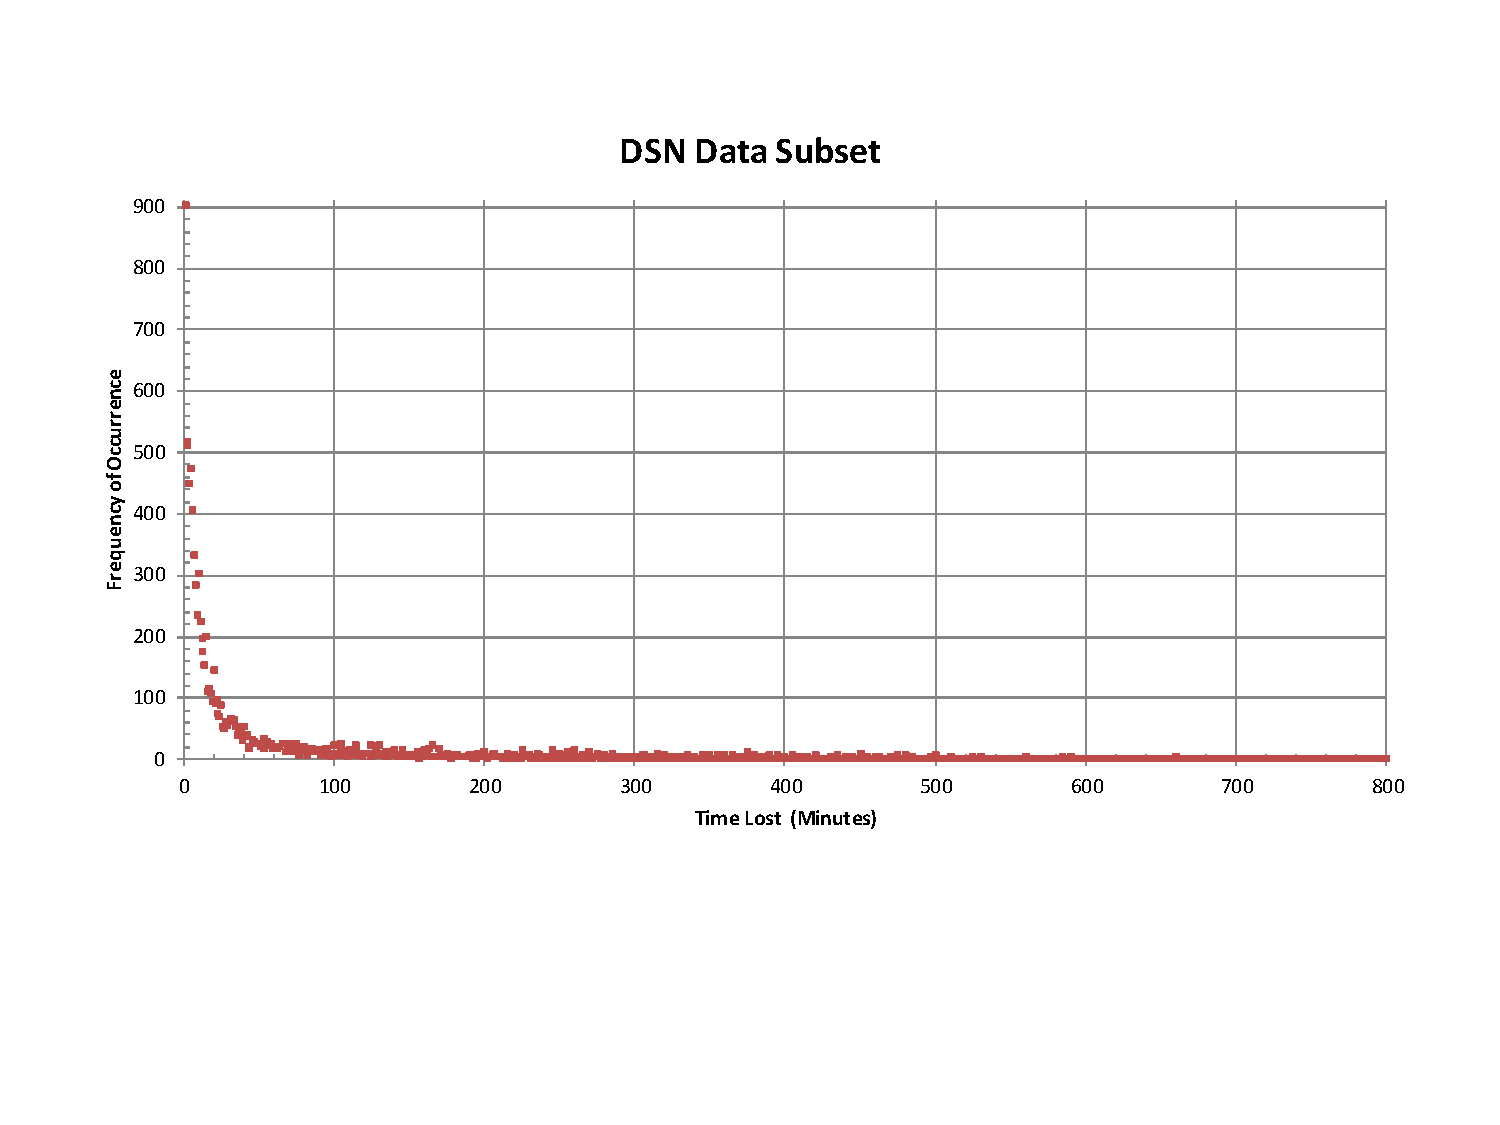
\includegraphics[width=8cm]{C:/Users/bornhi-t410/Documents/GitHub/piperResearch/figures2}
\caption{This is a plot of the presumably representative subset of DSN event data  provided to me, excluding events where no telemetry service was lost (or at least much less than one minute was lost) so that the shape of the curve that is seemingly traced out by the data plot can be seen with the naked eye.\label{fig:freqdist}}
\end{figure}

The following was our attempt to calculate the skewness of the DSN data:
$$ \gamma_1 = \frac{E[(X - \mu)^3]}{(E[(X - \mu)^2])^{3/2}} \approx 10.497 $$

After attempting to calculate the skewness of the data, and obtaining a positive value, we determined that this data could not possibly tend toward a normal distribution. We then attempted to fit the DSN data to a variety of other distributions, including some invented solely for this purpose. Unfortunately, none of these normalizable distributions quite fit with the data. Eventually a function was found that did seem to fit the data if the cases in which there was no telemetry loss were ignored. It seemed reasonable that perhaps this point was an outlier and could simply be omitted. Unfortunately, although it was possible to fit the data to a curve, this curve happened to be a variant of the hyperbolic cosine or hyperbolic cosecant functions, neither of which is normalizable over any reasonable intervals.

Even though we were not able to fit the DSN data to a continuous distribution, we were able to make headway using slightly less elegant numerical methods, which, in general, are better suited to deal with discrete probability distributions. We devised these methods in ways which were both easily implementable in SQL and very general. These methods can be easily modified to answer a wide range of additional questions which may be asked in the future. We were able to calculate all of the required information with relative ease.

Originally, we wrote functions to calculate the number of events, number of failures, probability of failure, probability of data loss, average telemetry loss, and ninety-fifth percentile telemetry loss for each given assembly. After realizing that it would be advantageous to devise these methods in a more genral form, we  modified these functions to receive assemblies, antennas, DSN complexes, or missions, and calculate the same statistics. For the purposes of making graphical representations of the query results, we realized that it would be useful to calculate the fifth percentile of telemetry loss values as well as the ninety-fifth, so that we could use error bars to show the range that ninety percent of the data fell into, which helped to give a sense of how uniform the losses due to failures were for a particular component. As a result of this realization, we generalized my ninety-fifth percentile function to return any given percentile’s value (Appendix A). The concepts behind relational databases and the tools afforded SQL language made the implementation of such methods relatively simple. As a result, the original goals of our project were accomplished in a considerably shorter amount of time than was expected.

%%%%%%%%%%%%%%%%%%%%%%%%%%%%%%%%%%%%%%%%%%%%%%%%%%%%%%%%%%%%%%%%%%%%%%%%%%%%%5

\section{Robust and Cost Effective Software Solutions}

Upon the completion of the original project goals we explored methods for making the DSN software more robust to failures given that software is a large contributor to service interuptions. We turned to the language of Erlang since we felt that it might have significant advantages, at least in this context due to its OTP Design Principles, over other solutions given that Erlang was designed to respond to the requirements of telecommunication system applications. \cite{armstrong2003}

\begin{figure}[h]
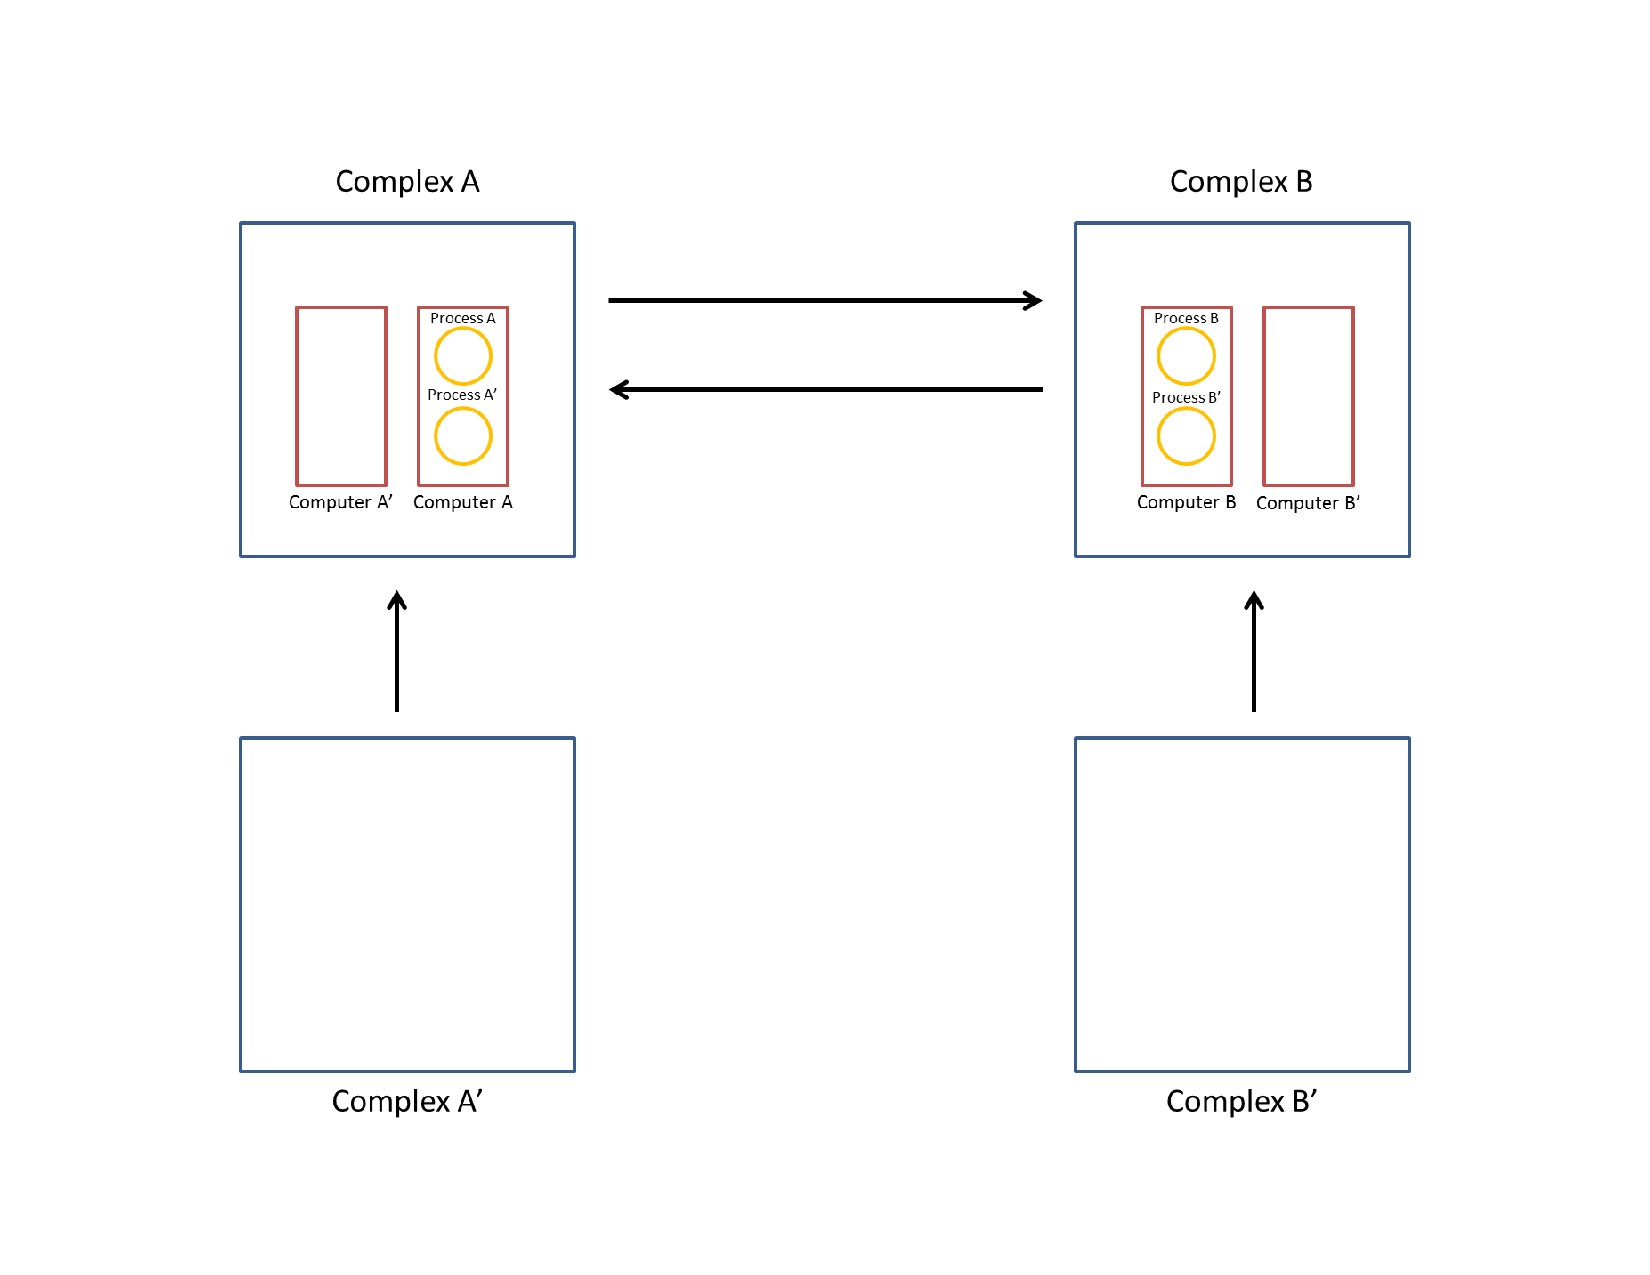
\includegraphics[width=8cm]{C:/Users/bornhi-t410/Documents/GitHub/piperResearch/diagram}
\caption{This is a diagram of our particular conceptual implementation of the OTP Design Principles to work with the DSN. \label{fig:diagram}}
\end{figure}

The main concept of our procedures is illustrated in Figure~\ref{fig:diagram}. Two different locations which are part of the DSN (labeled as $Complex A$ and $Complex B$ in Figure~\ref{fig:diagram}) can directly communicate with one another. In the case of an error at $Complex A$, our concept entails that $Complex B$ should not be affected, or even otherwise be aware of the failure. The idea is that there should be another process already running ($Process A^\prime$) which is capable of seamlessly taking over without losing any information in transit between $Complex A$ and $Complex B$. Using the OTP Design Principles The information in transit can be put into a queuing process which can store the information until $Process A^\prime$ has successfully taken over the responsibilities of $Process A$. \cite{cesarini2009} Furthermore, if for some reason $Computer A$ has a hardware malfunction, or some other kind of irrecoverable failure, $Computer A^\prime$ should be ready and able to seamlessly take over. This can even be implemented on a larger scale by completely separate complexes. If $Complex A$ suffers a fatal error, $Complex A^\prime$ can take over without disturbing $Complex B$ at all. This methodology need not be limited to one back-up system at each level. It may be prudent in many cases to have $Process A^{\prime \prime}$ or even $Process A^{\prime \prime \prime}$ in situations in which errors are particularly likely.

All of these things can be accomplished within the framework provided by the OTP framework of Erlang using its distributed programming implementation with supervisor processes. \cite{logan2011} When a child process encounters an irrecoverable error it notifies its supervisor and ends itself. Its supervisor can then restart the child process. When a supervisory process encounters an error it stops all of its child processes and then itself. This behaviour can be modified to cause the supervisor to start a new version of itself before stopping, which would then go on to respawn its child processes. This kind of a framework allows for very robust networking which is capable of isolating and eliminating problems quickly, efficiently, and, most importantly, without affecting the rest of the network.

%%%%%%%%%%%%%%%%%%%%%%%%%%%%%%%%%%%%%%%%%%%%%%%%%%%%%%%%%%%%%%%%%%%%%%%%%%%%%

\section{Conclusions}

During the course of this project failures of the DSN were investigated. Using a subset of historical DSN event data as a statistical case study, general SQL queries were developed and tested for extracting meaningful information from the overwhelming amount of raw data generated by the DSN. The original intent of this investigation was simply to provide the DSN administration with quantitative measurements of the DSN's shortcomings, as well as to arm them with the tools to easily reassess the DSN in the future. This goal was accomplished.

The project then evolved into an exploration of the applicability of the Erlang language OTP framework to the design of more robust DSN software solutions. Time did not allowed for a direct comparison between Erlang and alternative architectures written in Java or C/C++ which are currently the languages primarily used in the DSN.  However, the authors of this paper are fairly confident that Erlang provides a viable option for the design and implementation of selective applications within the DSN software infrastructure.  

%%%%%%%%%%%%%%%%%%%%%%%%%%%%%%%%%%%%%%%%%%%%%%%%%%%%%%%%%%%%%%%%%%%%%%%%%%%%%%
%% Place all of the references you used to write this paper in a file
%% with the same name as following the \bibliography command
%%%%%%%%%%%%%%%%%%%%%%%%%%%%%%%%%%%%%%%%%%%%%%%%%%%%%%%%%%%%%%%%%%%%%%%%%%%%%%

\bibliography{sample-paper}

\bibliographystyle{prsty}
\begin{thebibliography}{99}
\bibitem{bagri2007}Bagri, D.S., Statman, J.I., Gatti, M., in \textit{Proceedings of the IEEE}, vol. 95, no. 10, Pasadena,  2007.
\bibitem{wackley2011}Wackley, J., Dundics, D., The Interplanetary Network Progress Report 41-187, 2011.
\bibitem{armstrong2003}Armstrong, J., Ph.D. thesis, Royal Institute of Technology, Stockholm, Sweden, 2003.
\bibitem{logan2011}Logan, M., Merritt, E., Carlsson, R., \textit{Erlang and OTP In Action} (Manning Publications Co., Stamford, CT, 2011).
\bibitem{cesarini2009}Cesarini, F., Thompson, S., \textit{Erlang Programming} (O'Reilly Media, Inc., Sebastopol, CA, 2009).
\end{thebibliography}


%%%%%%%%%%%%%%%%%%%%%%%%%%%%%%%%%%%%%%%%%%%%%%%%%%%%%%%%%%%%%%%%%%%%%%%%%%%%%%

\begin{acknowledgments} 
This work was supported by the California Institute of Technology and the National Aeronautics and Space Administration. I.B. thanks Harihar Subramanyam, Cecilia Sanders, and Michael Younkin for their technical assistance, as well as David Mohr for his guidance and unreasonable kindness.
\end{acknowledgments}

%%%%%%%%%%%%%%%%%%%%%%%%%%%%%%%%%%%%%%%%%%%%%%%%%%%%%%%%%%%%%%%%%%%%%%%%%%%%%%
\clearpage
\appendix

\section{Query Results for a Sample Data Set}

\begin{figure}[h]
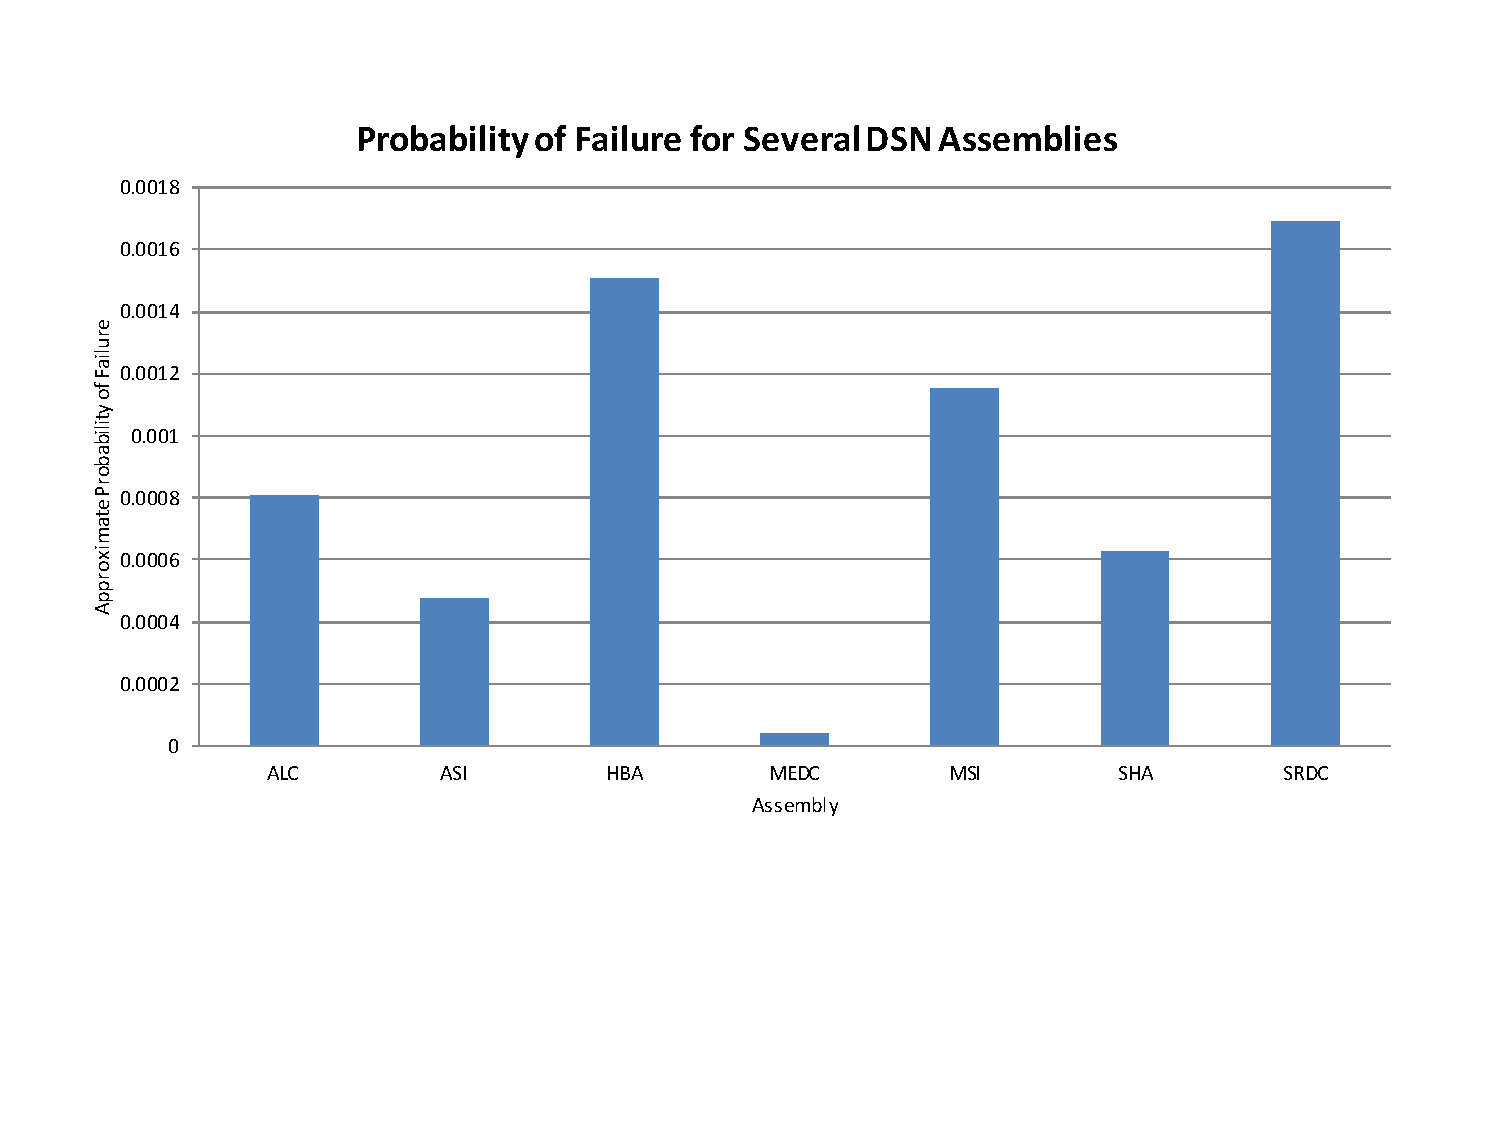
\includegraphics[width=8cm]{C:/Users/bornhi-t410/Documents/GitHub/piperResearch/probOfFailureAssembly}
\caption{This graph displays the probability of failure for several DSN assemblies.\label{fig:fig2}}
\end{figure}

\begin{figure}[h]
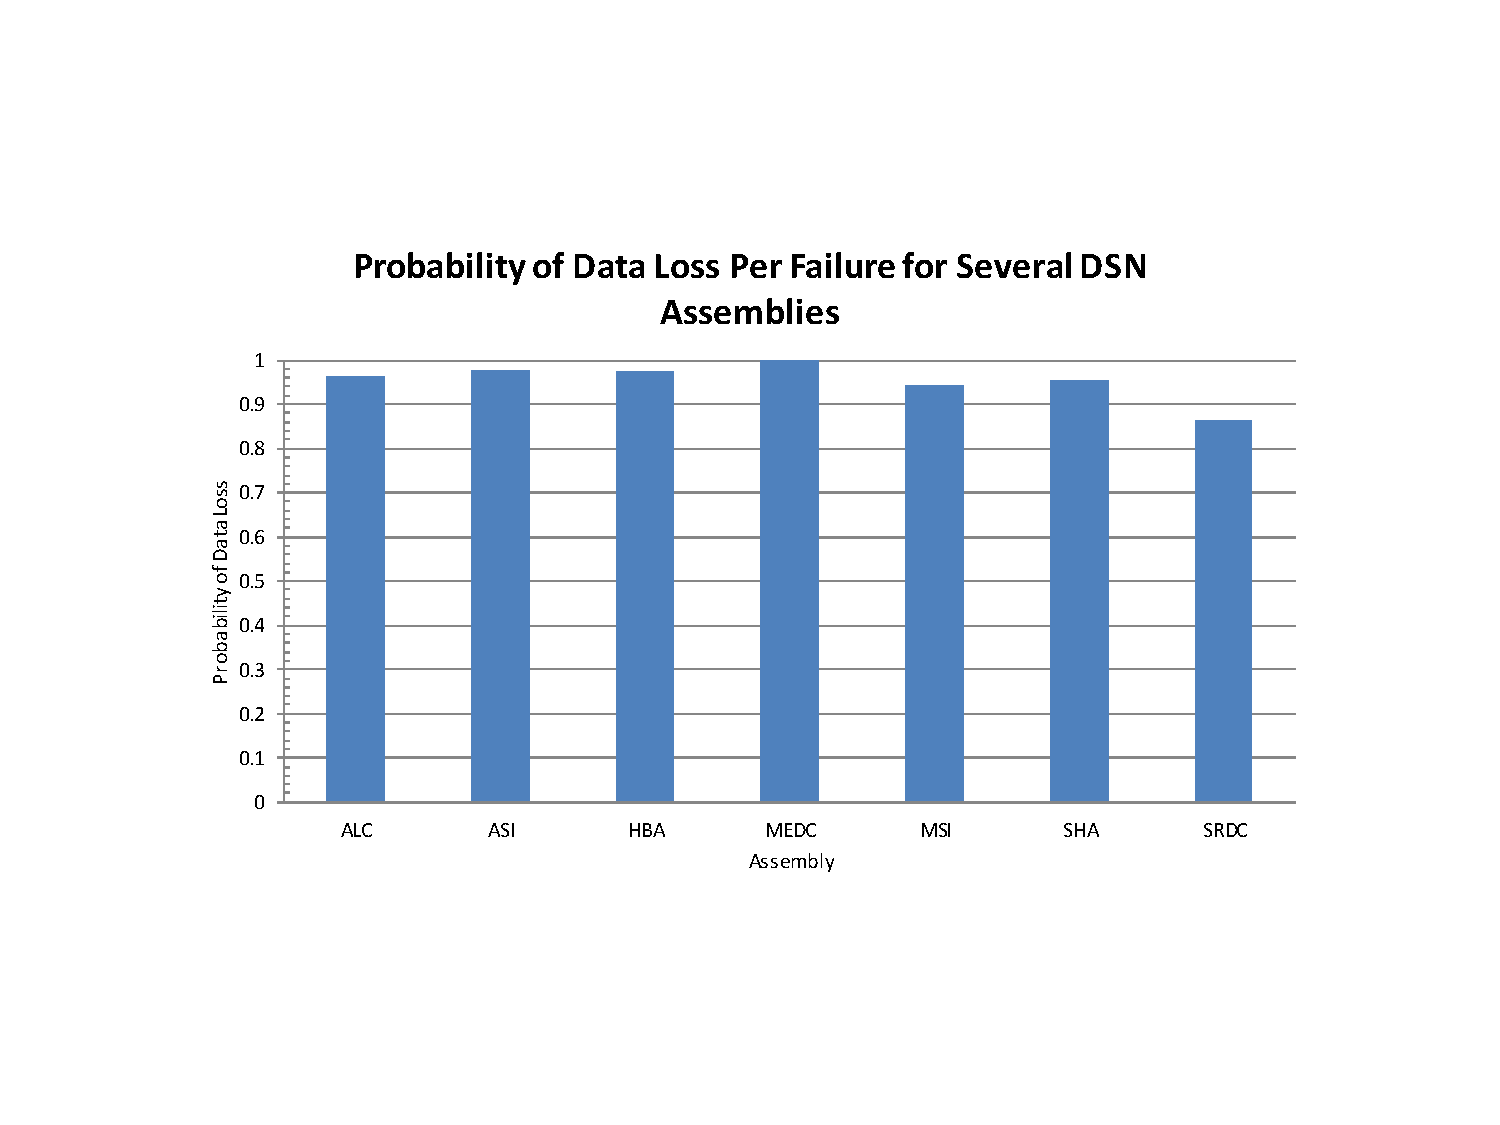
\includegraphics[width=8cm]{C:/Users/bornhi-t410/Documents/GitHub/piperResearch/probOfLossAssembly}
\caption{This graph displays the probability of data loss per failure for several DSN assemblies.\label{fig:fig3}}
\end{figure}

\begin{figure}[h]
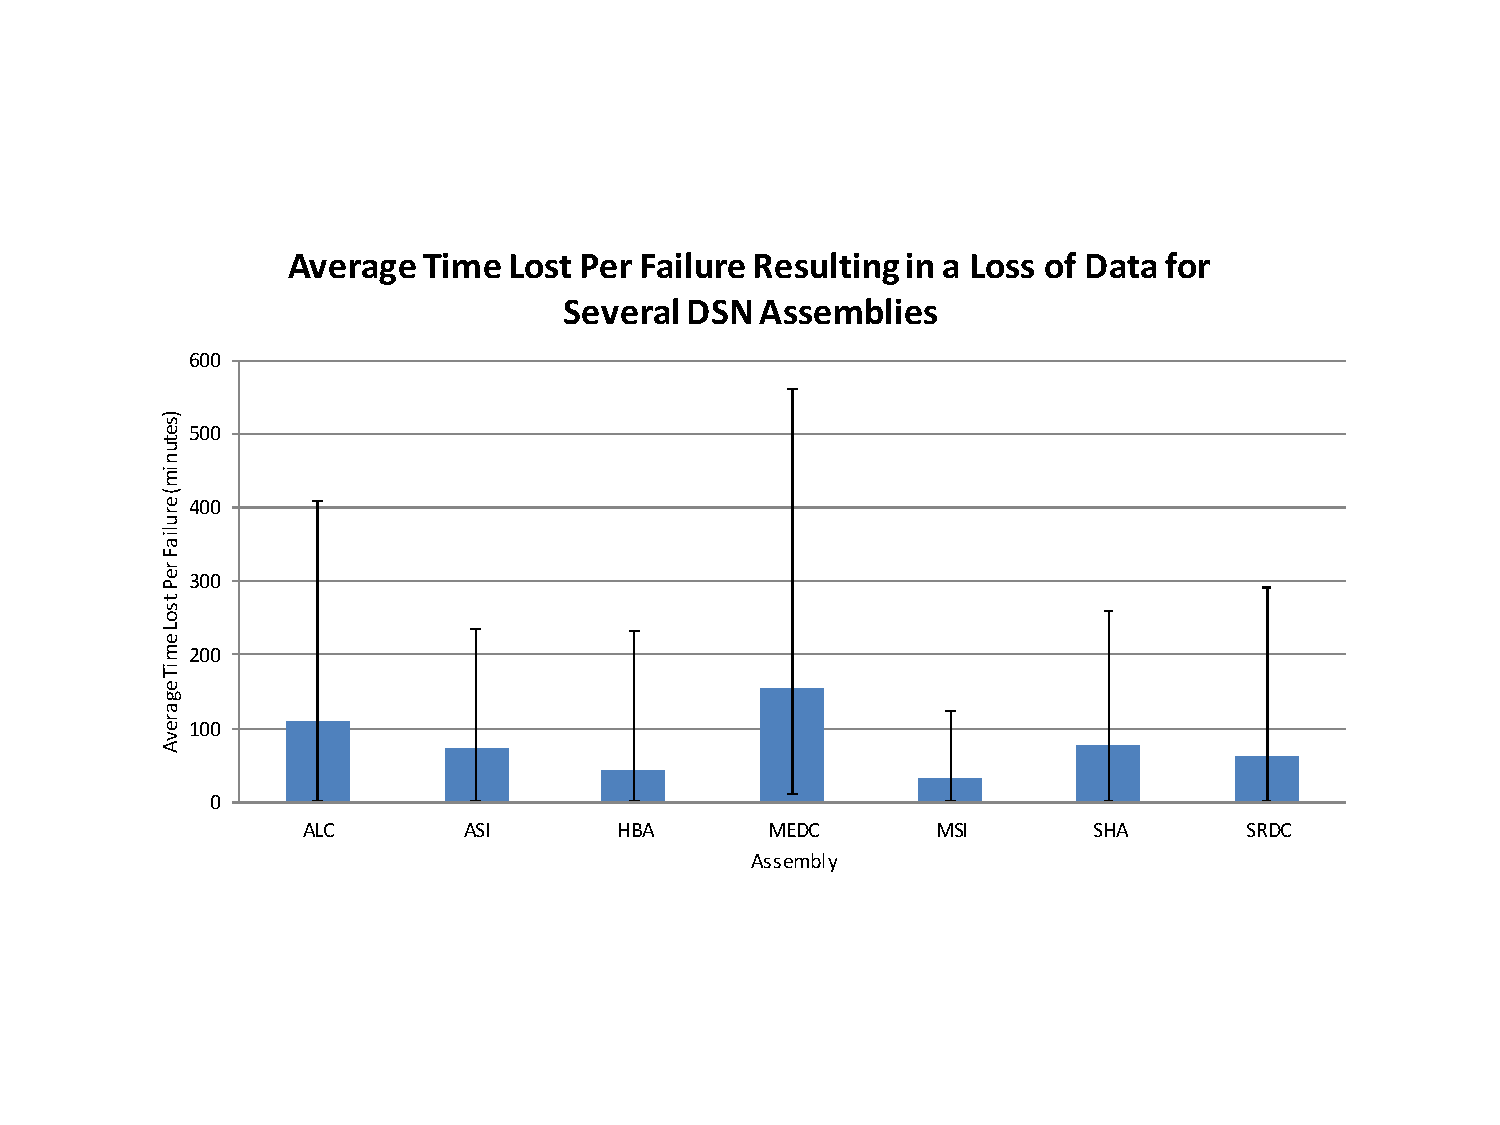
\includegraphics[width=8cm]{C:/Users/bornhi-t410/Documents/GitHub/piperResearch/avgFailureAssembly}
\caption{This graph displays the average data loss per failure resulting in data loss for several DSN assemblies in minutes. The error bars denote the $5^{th}$ and $95^{th}$ percentile values. \label{fig:fig4}}
\end{figure}

\begin{figure}[h]
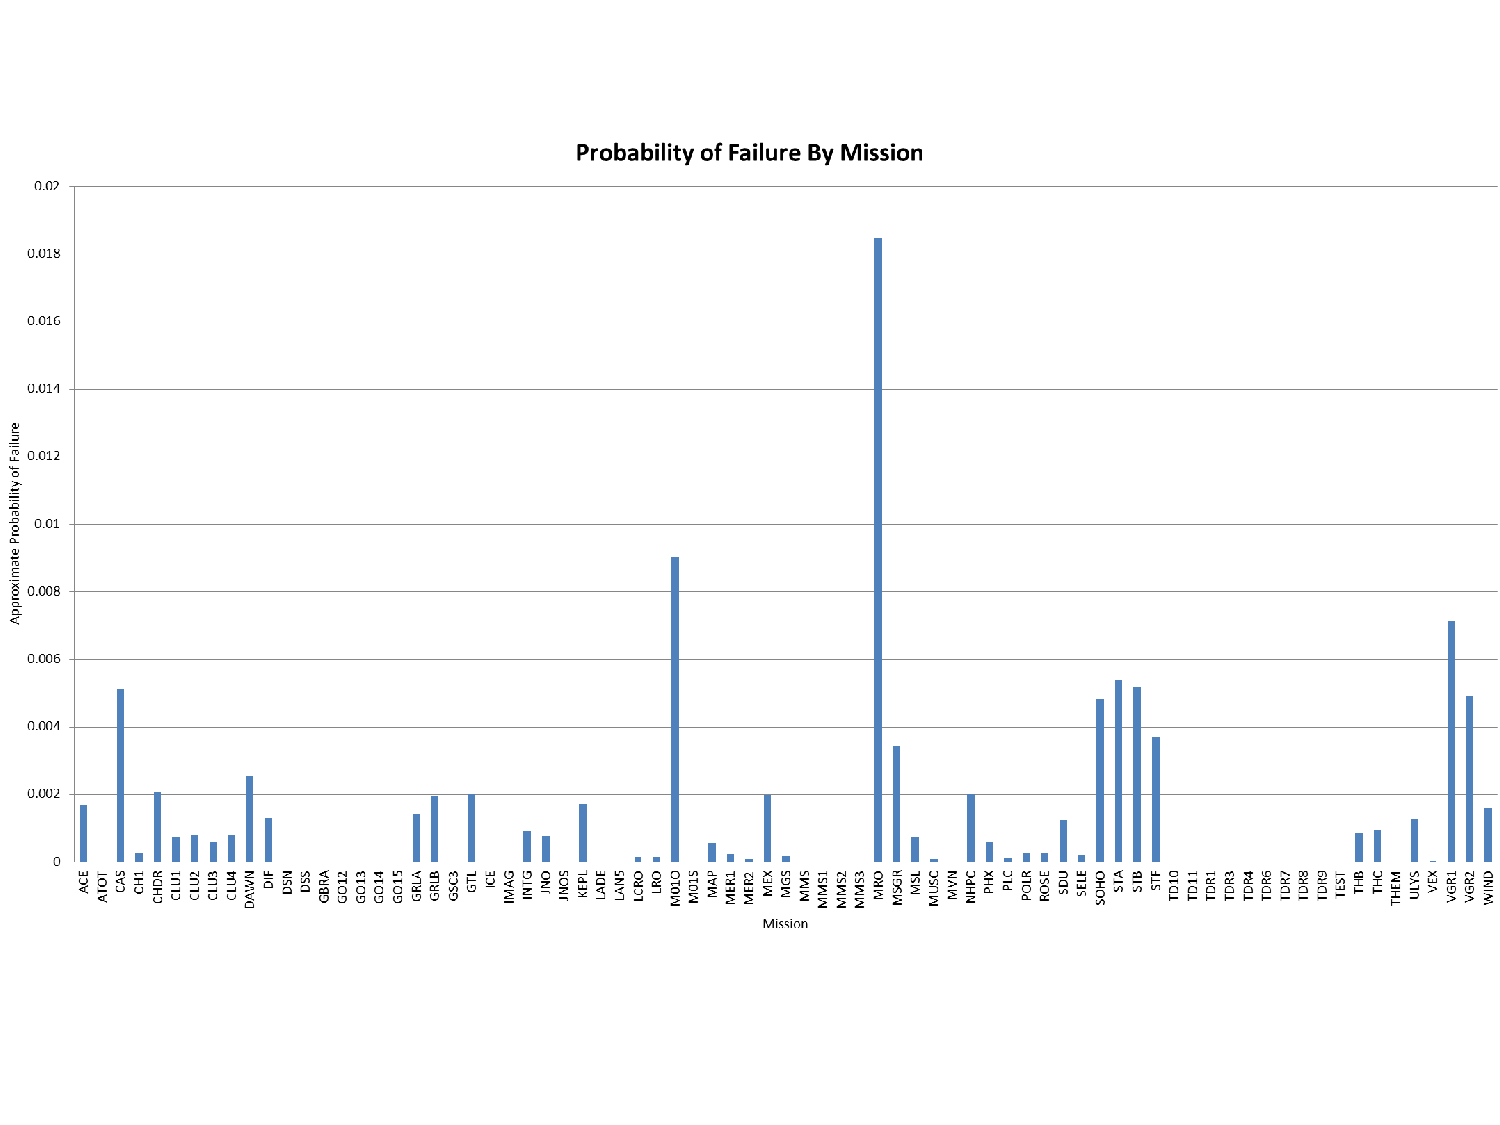
\includegraphics[width=8cm]{C:/Users/bornhi-t410/Documents/GitHub/piperResearch/probOfFailureMission}
\caption{This graph displays the probability of failure by DSN mission.\label{fig:fig5}}
\end{figure}

\begin{figure}[h]
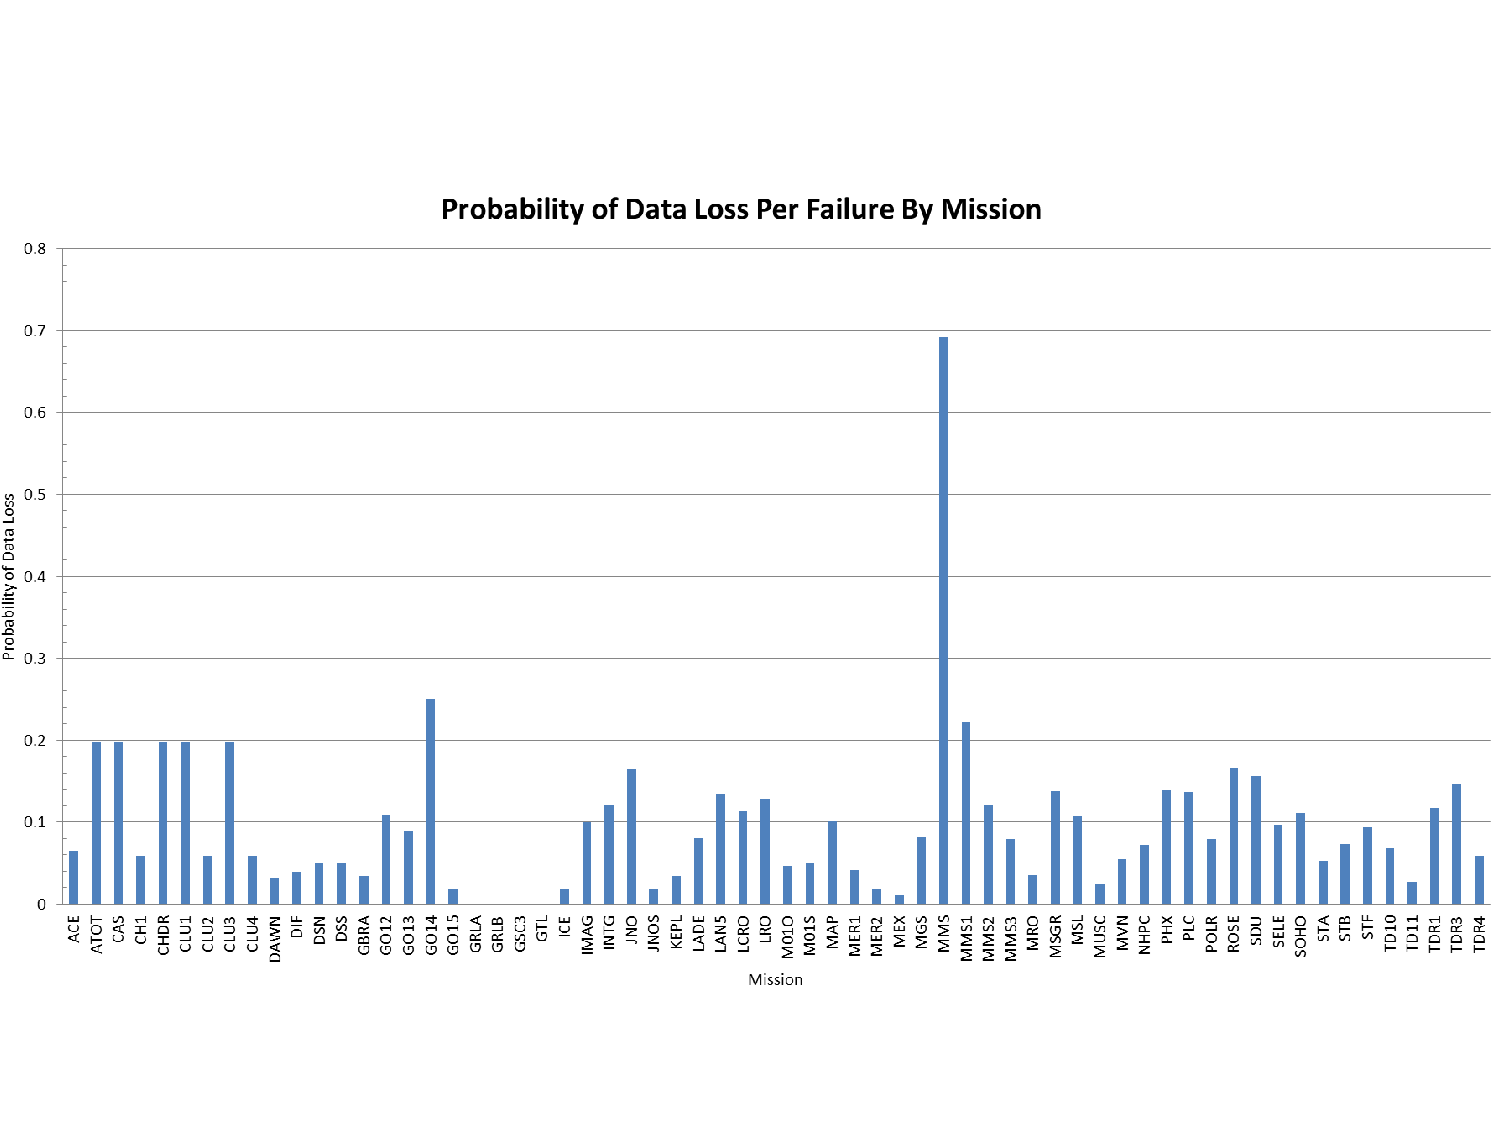
\includegraphics[width=8cm]{C:/Users/bornhi-t410/Documents/GitHub/piperResearch/probOfLossMission}
\caption{This graph displays the probability of data loss per failure by DSN mission.\label{fig:fig6}}
\end{figure}

\begin{figure}[h]
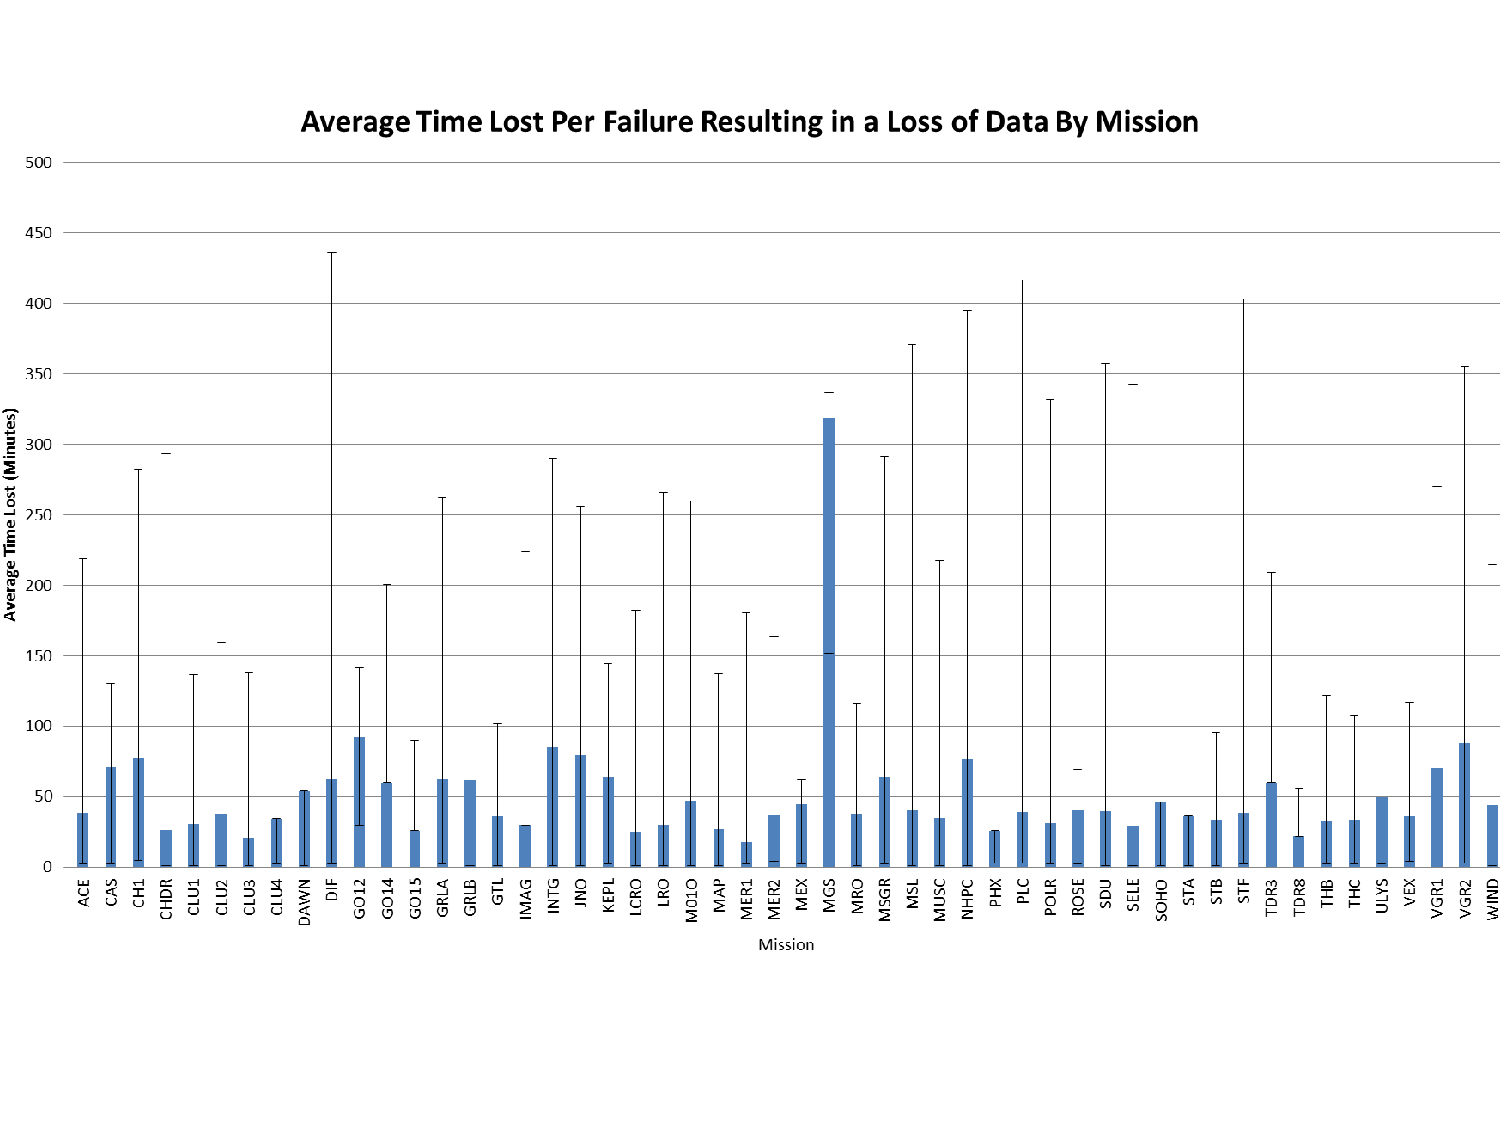
\includegraphics[width=8cm]{C:/Users/bornhi-t410/Documents/GitHub/piperResearch/avgFailureMission}
\caption{This graph displays the average data loss per failure resulting in data loss by DSN mission in minutes. The error bars denote the $5^{th}$ and $95^{th}$ percentile values. \label{fig:fig7}}
\end{figure}

\begin{figure}[h]
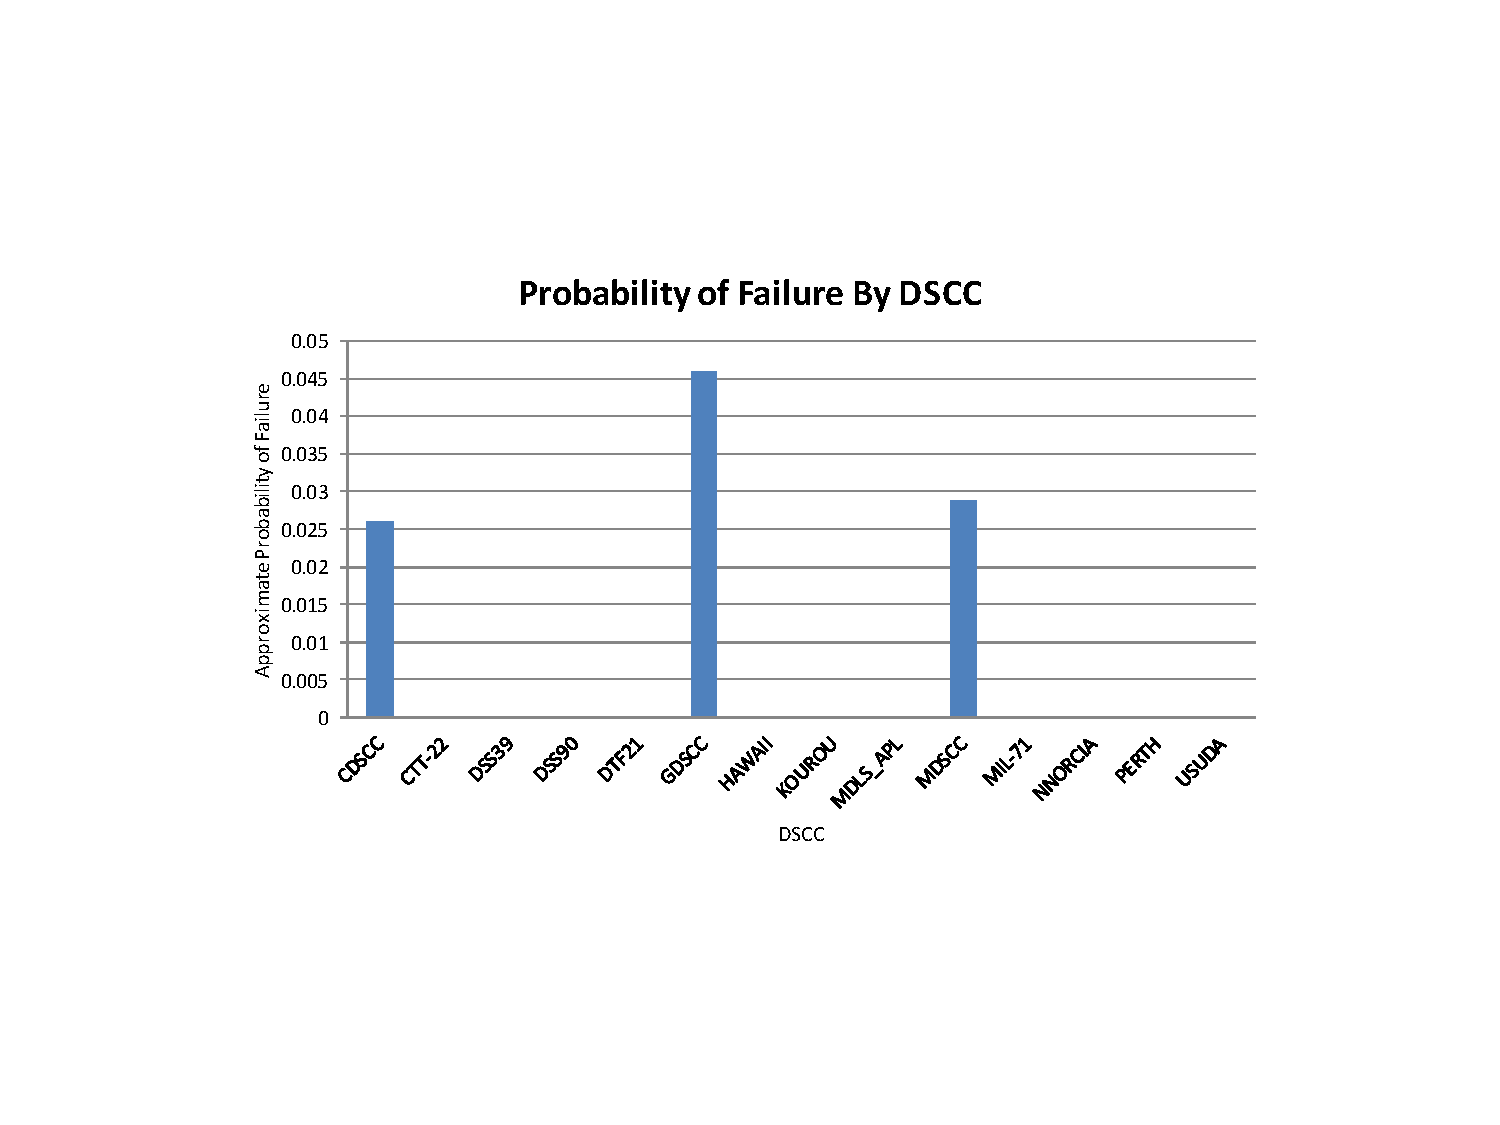
\includegraphics[width=8cm]{C:/Users/bornhi-t410/Documents/GitHub/piperResearch/probOfFailureDscc}
\caption{This graph displays the probability of failure by DSCC.\label{fig:fig8}}
\end{figure}

\begin{figure}[h]
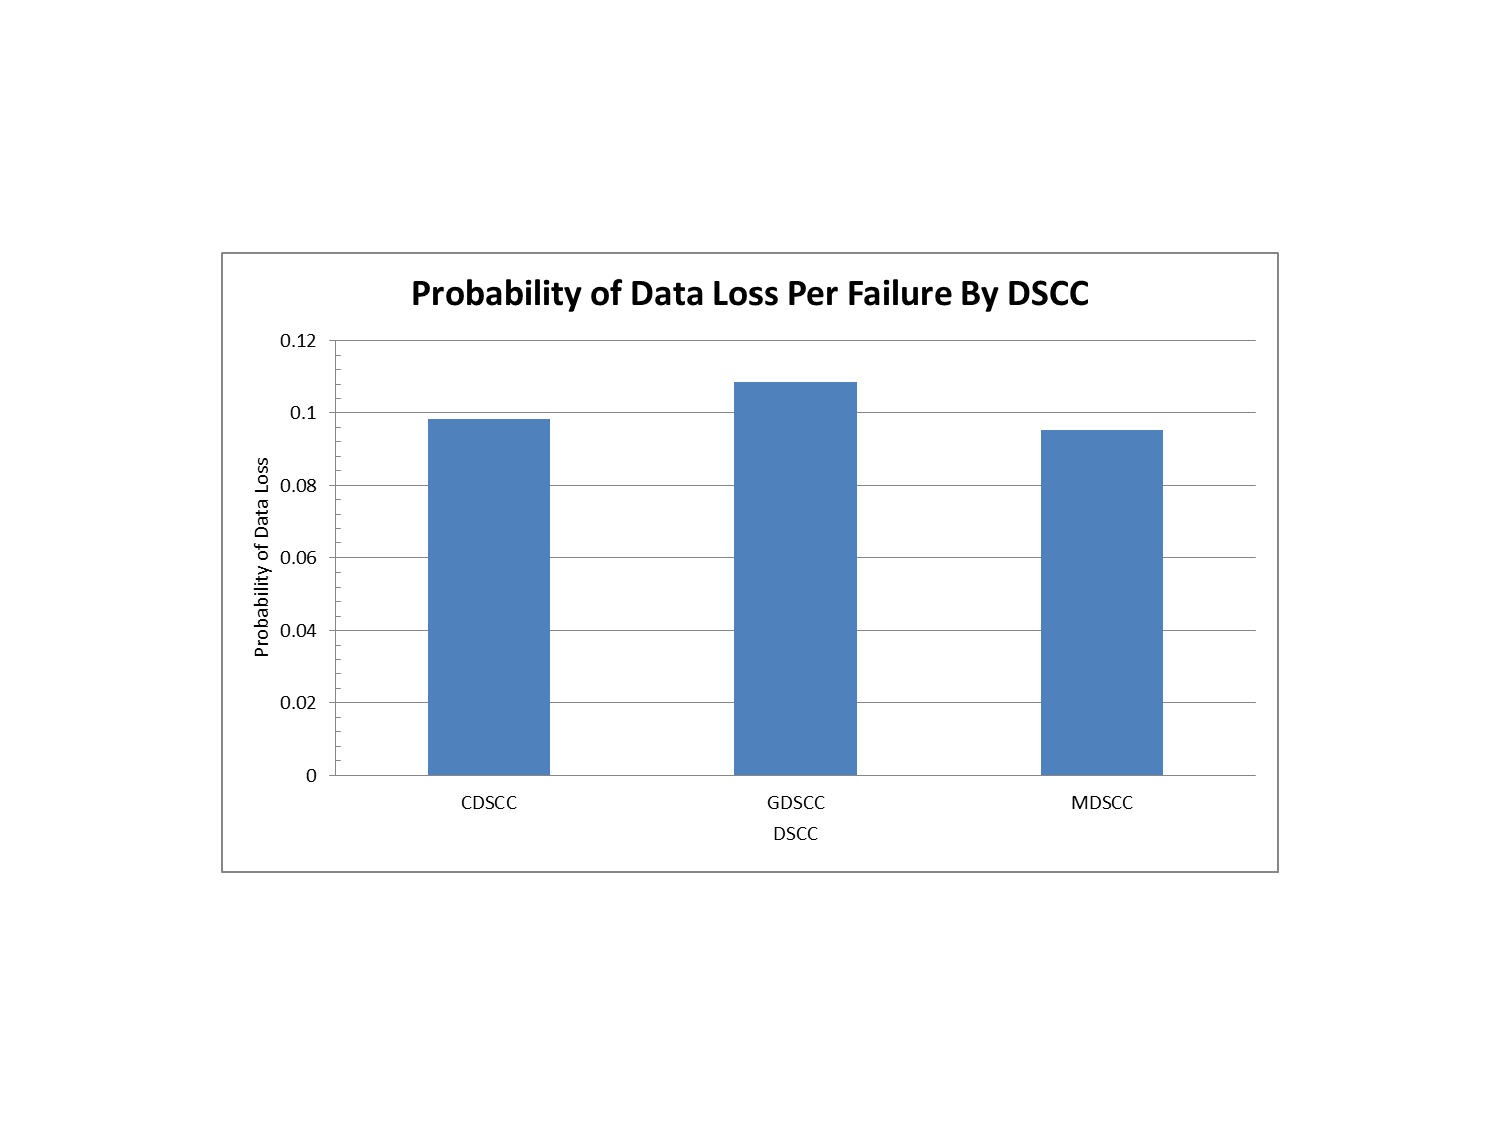
\includegraphics[width=8cm]{C:/Users/bornhi-t410/Documents/GitHub/piperResearch/probOfLossDscc}
\caption{This graph displays the probability of data loss per failure by DSCC. \label{fig:fig9}}
\end{figure}

\begin{figure}[h]
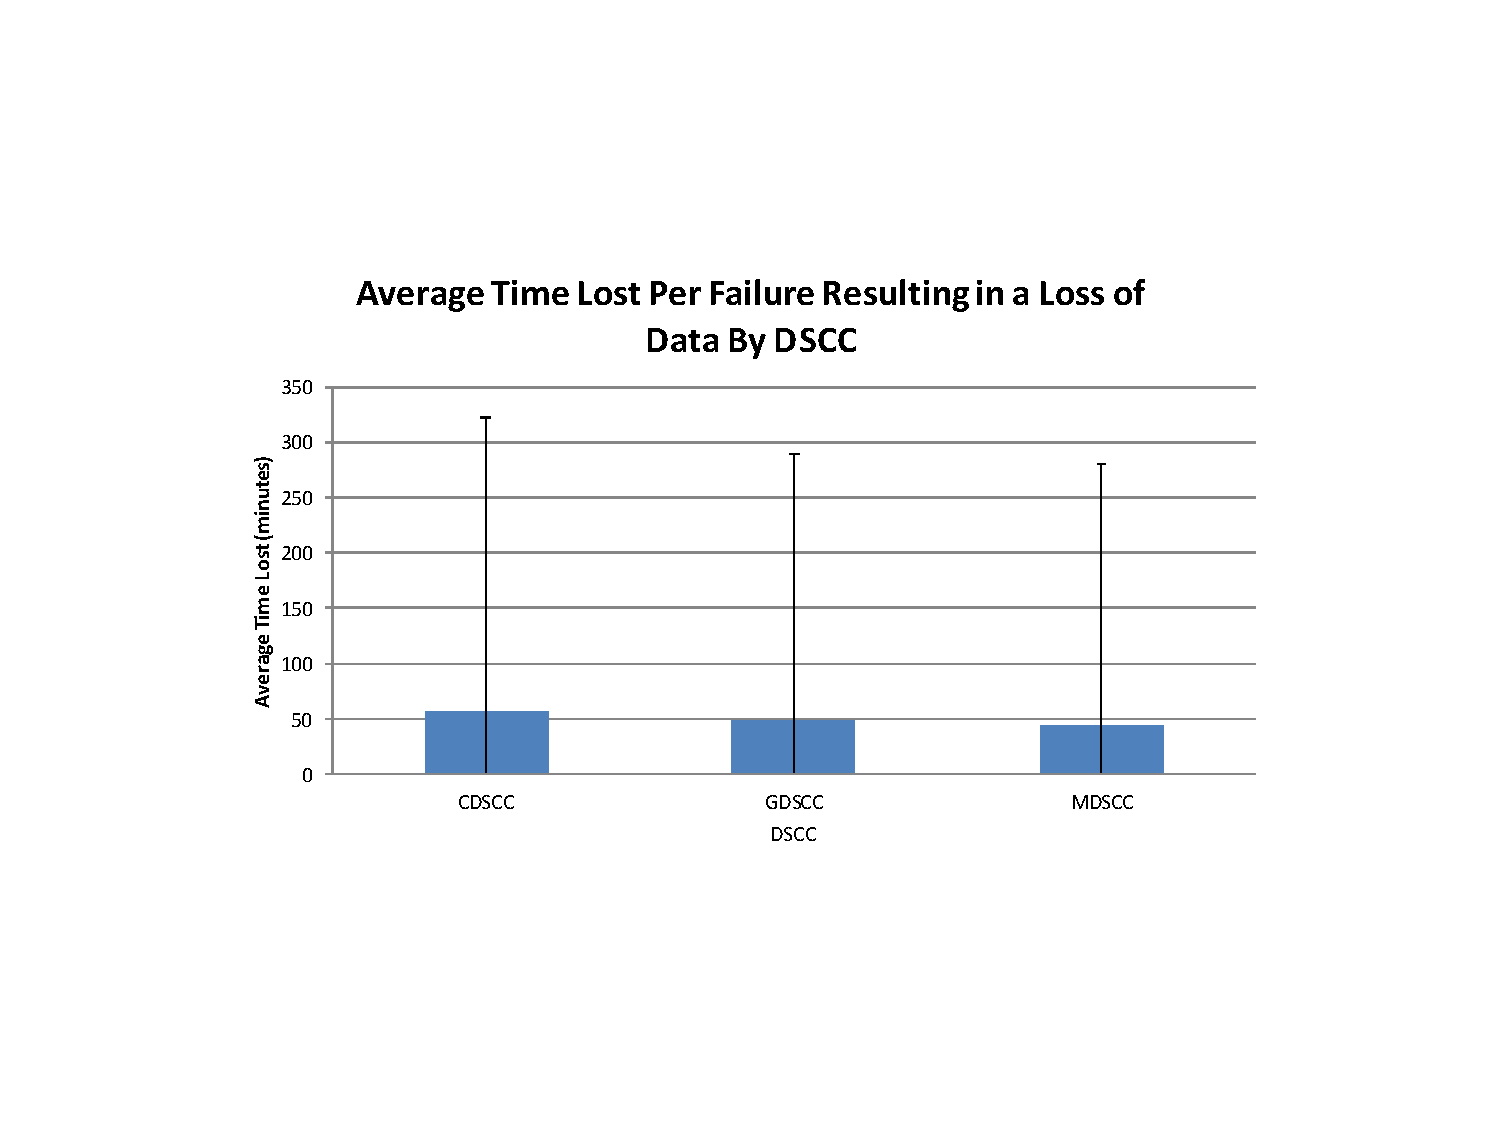
\includegraphics[width=8cm]{C:/Users/bornhi-t410/Documents/GitHub/piperResearch/avgFailureDscc}
\caption{This graph displays the average data loss per failure resulting in data loss by DSCC in minutes. The error bars denote the $5^{th}$ and $95^{th}$ percentile values. \label{fig:fig10}}
\end{figure}

\begin{figure}[h]
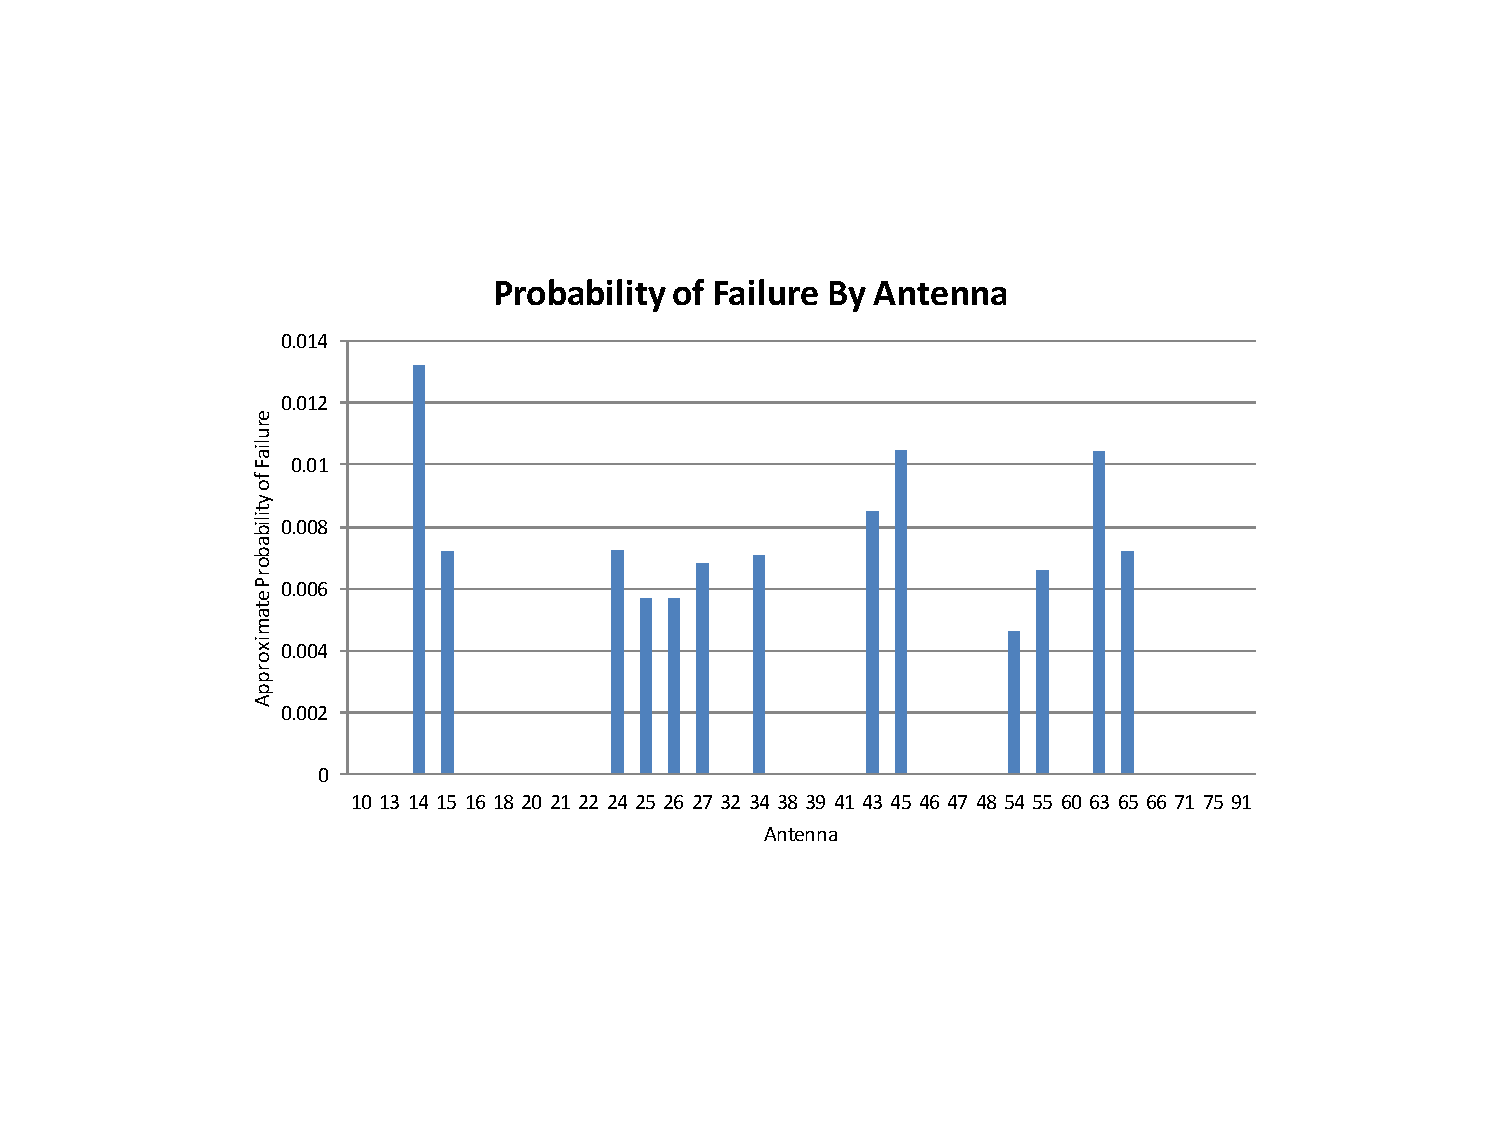
\includegraphics[width=8cm]{C:/Users/bornhi-t410/Documents/GitHub/piperResearch/probOfFailureAntenna}
\caption{This graph displays the probability of failure by DSN antenna.\label{fig:fig11}}
\end{figure}

\begin{figure}[h]
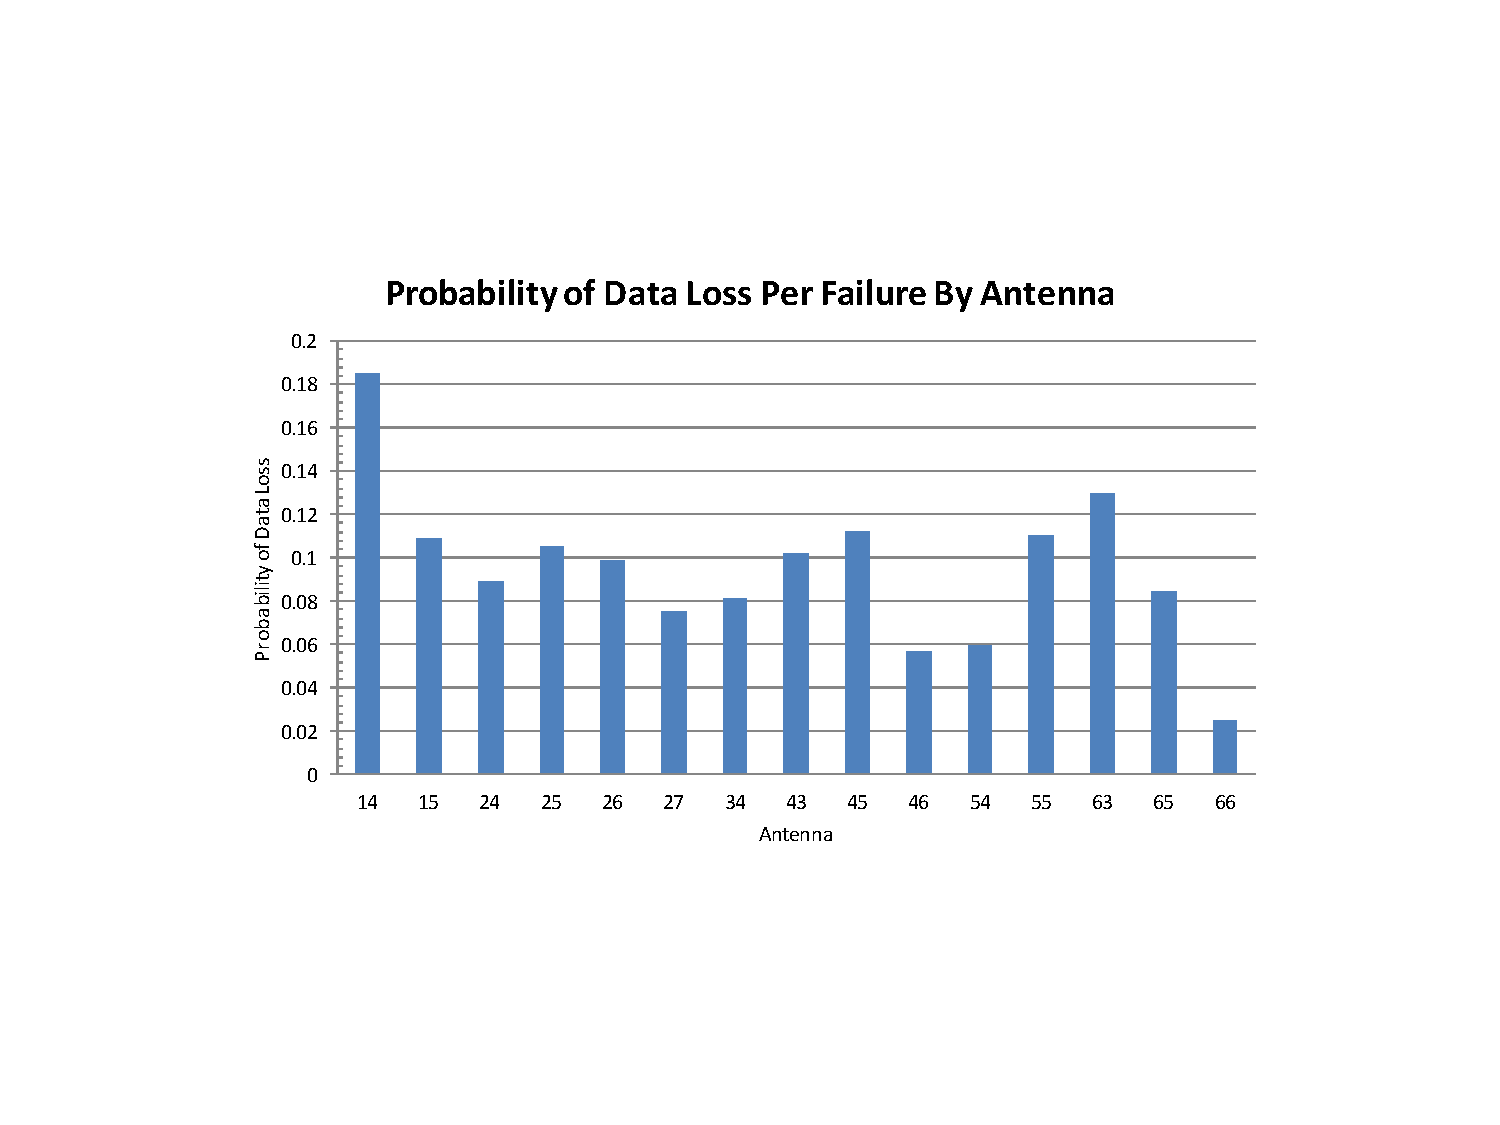
\includegraphics[width=8cm]{C:/Users/bornhi-t410/Documents/GitHub/piperResearch/probOfLossAntenna}
\caption{This graph displays the probability of data loss per failure by DSN antenna. \label{fig:fig12}}
\end{figure}

\begin{figure}[h]
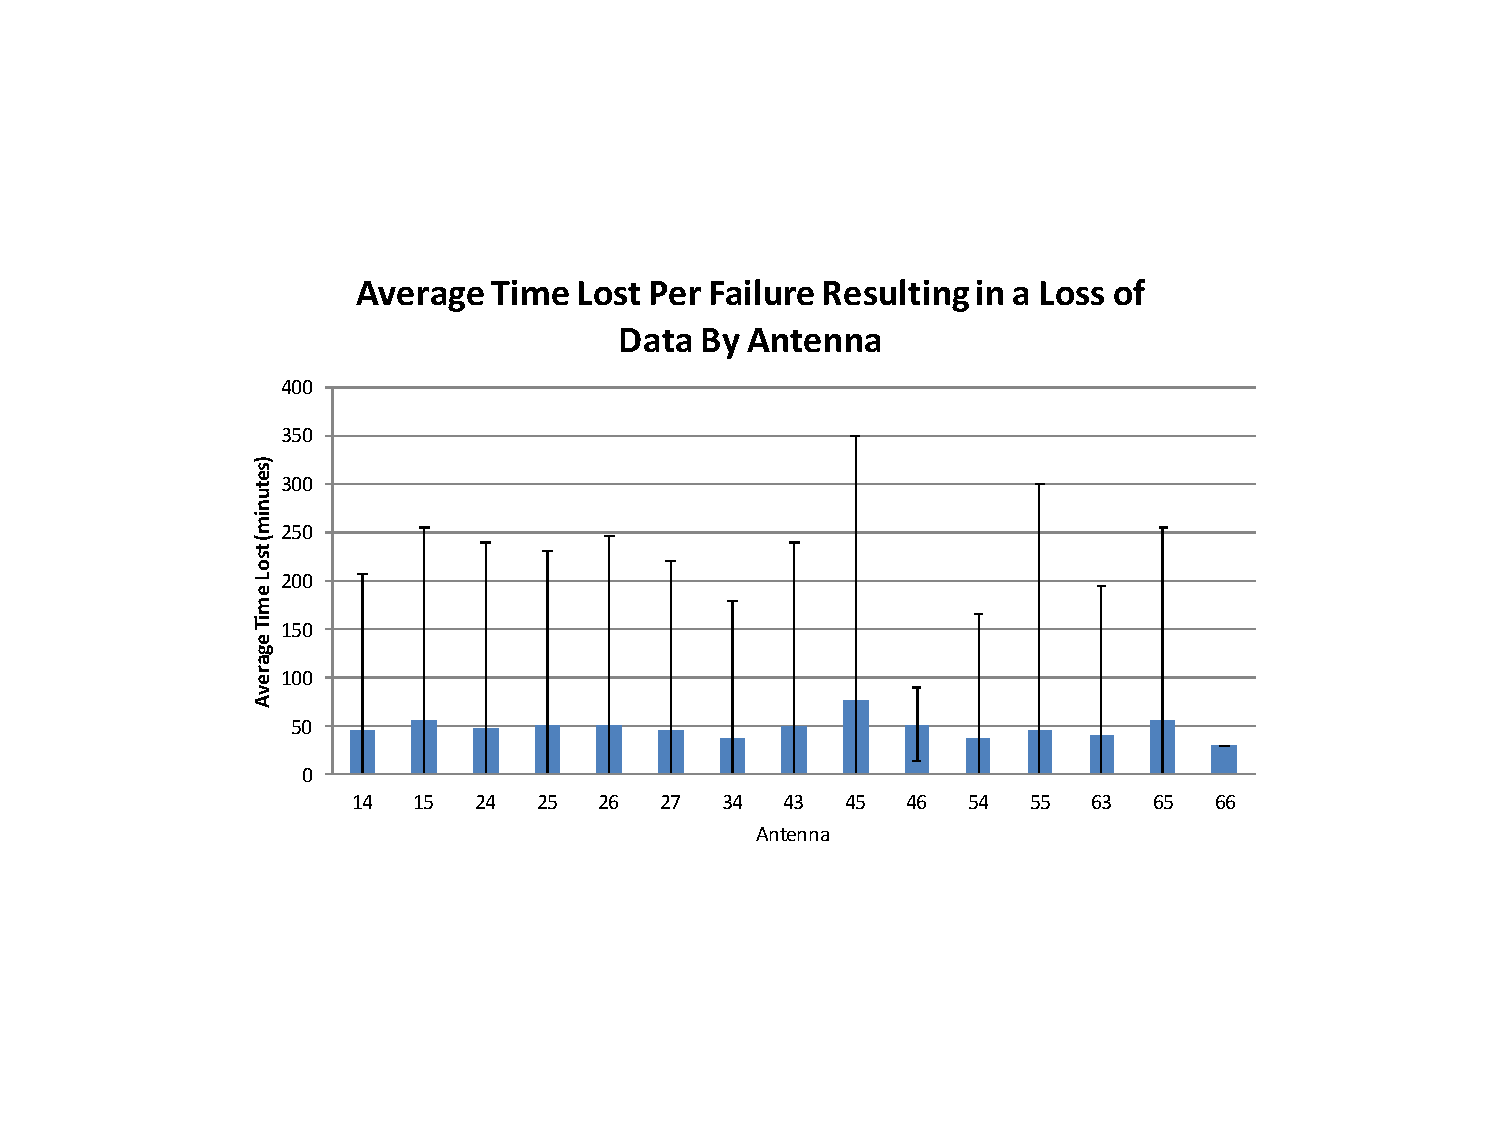
\includegraphics[width=8cm]{C:/Users/bornhi-t410/Documents/GitHub/piperResearch/avgFailureAntenna}
\caption{This graph displays the average data loss per failure resulting in data loss by DSN antenna in minutes. The error bars denote the $5^{th}$ and $95^{th}$ percentile values. \label{fig:fig13}}
\end{figure}

\end{document}
